\chapter{Characterizing and mitigating terrestrial noise sources} \label{c:DetChar}

\section{Characterizing general transient noise } 

Event trigger generators, or ETGs, are essential tools for evaluating transient noise in auxiliary channels, including seismic channels. ETGs identify periods of excess signal, often referred to as \textit{glitches}, and calculate useful characteristics about these features like central time, central frequency, and amplitude.

\subsection{Performance of single interferometer burst pipelines}
The ETG Omicron, which I have chosen to use for seismic transients studies for reasons shown in Figure \ref{fig:ETGs}, works by the following procedure: 
\begin{enumerate}
\item Data is projected onto a sine-gaussian basis via tiling in time, frequency, and Q (number of cycles of the signal).
\item Data is whitened by the median-mean power spectral density (robust to transient noise pollution) 
for some time segment known as \textit{block duration}.
\item The most significant tile becomes an Omicron trigger with 
associated time, frequency, Q, and amplitude. 
\end{enumerate}

As an example of the studies performed so far, I compared the detection efficiency of different ETGs for a range of plausible \gw{} waveforms (sine gaussians, ring downs, and core-collapse supernovae waveforms generated with numerical simulations). Figure~\ref{fig:ETGs} shows that Omicron and Omega detect nearly 100\% of all injected signals, as expected. The study also showed that for detected signals, Omicron and Omega also outperform ExcessPower in reconstructing trigger parameters like central time and SNR. 
 
\begin{figure}[htb]
	\center{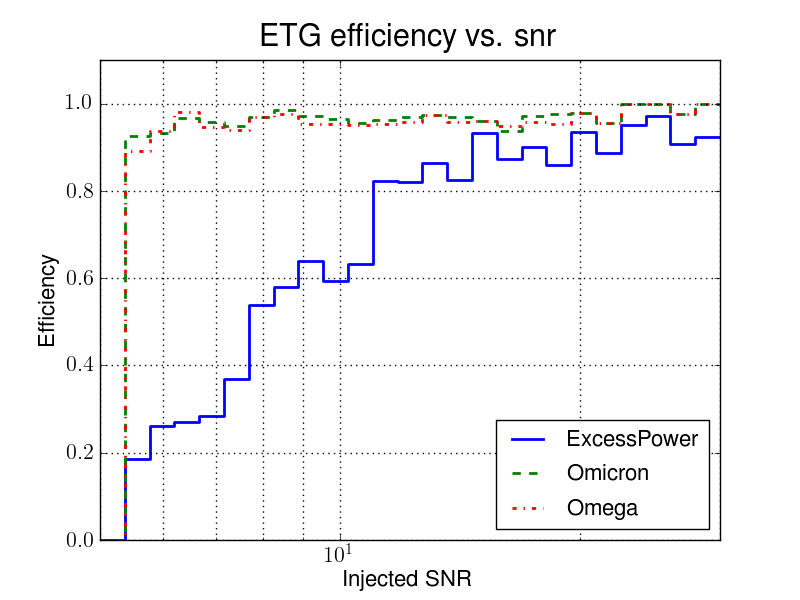
\includegraphics[scale=0.4]
	{figures/ER3_efficiency_vs_snr.png}}
	\caption{\label{fig:ETGs} Efficiency vs. SNR for the three algorithms that are being considered by the collaboration as potential single interferometer burst search pipelines (Omicron, Omega, and ExcessPower)}.
\end{figure}


We still need to optimize Omicron's running parameters for the identification of seismic noise transients at low frequency (0.1-10Hz), as previous ETG studies targeted the aLIGO search band (see Figure \ref{fig:ETGs}). 
A remaining hurdle, as shown in \cite{Macleod-Seisveto} is that ETGs require significant tuning away from their standard parameters in order to resolve the low frequency, long duration transients commonly seen in seismic sensors - see Figure \ref{fig:OmicronTuning} for an example of this. 
In terms of Omicron parameters, this will likely require using much longer block duration than the standard configuration of 32s for whitening, as we want enough data to resolve features that could potentially have durations of tens or hundreds of seconds. \todo{DONE?}


%
%%
%%%
\section{Seismic noise}

\subsection{Livingston train up-conversion} 


Seismic noise from the nearby train at Livingston was a common problem for transient \gw{} searches during the previous science run. 
We discovered that the 1-3Hz seismic noise produced by the train does couple into the PRMI Power Recycling Cavity Length signal (see Figure \ref{fig:aLIGOconfig}) at frequencies within the \gw{} search band (20-40Hz) - see Figure \ref{fig:TRAIN}). 
\todo{Replace all with DARM results!!}

\begin{figure}[htb]
\centering
\begin{subfigure}{.48\textwidth}
  \centering
  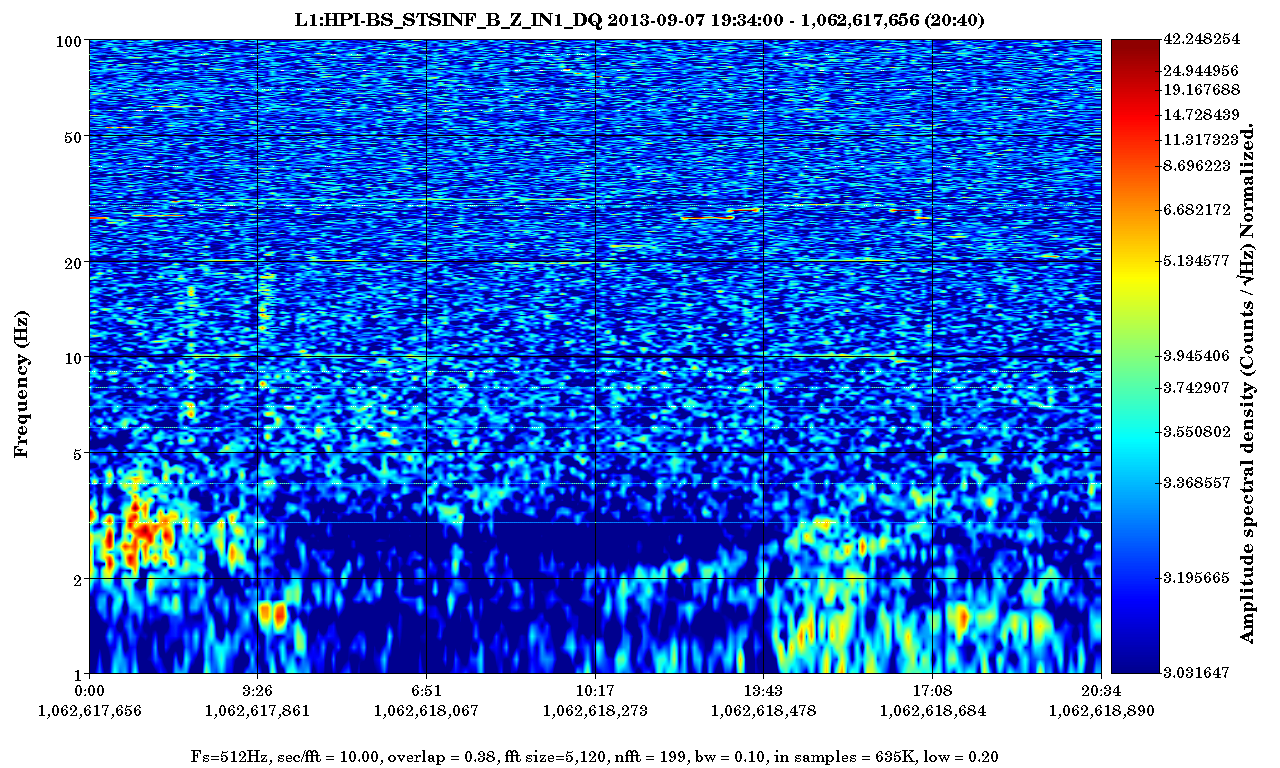
\includegraphics[width=\linewidth]{figures/GroundMotionSpec.png}
  \caption{Ground motion}
  \label{fig:TrainGroundSpec}
\end{subfigure}%
\begin{subfigure}{.48\textwidth}
  \centering
  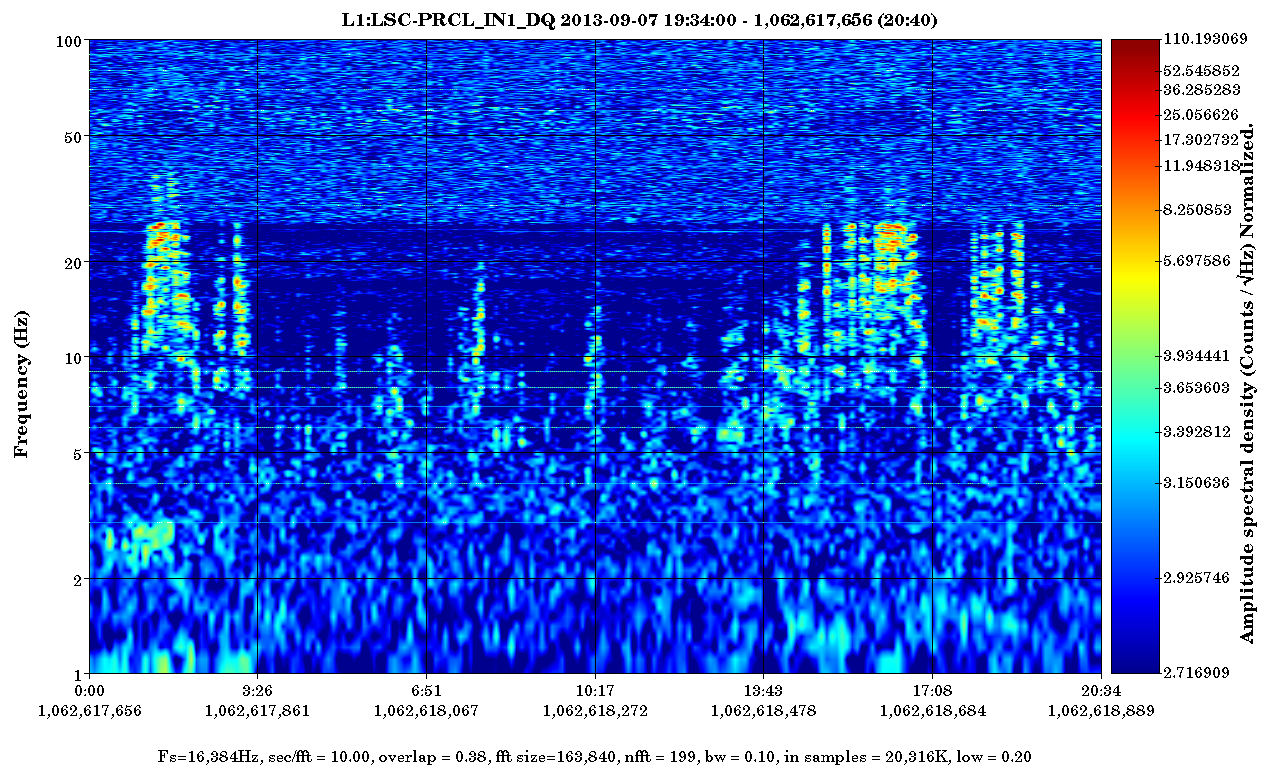
\includegraphics[width=\linewidth]{figures/PRMI_PRCL_spec.png}
  \caption{PRMI control signal}
  \label{fig:TrainPRCL}
\end{subfigure}
\caption{Normalized spectrograms of a recent 20 minute Livingston PRMI lock time during which a train was passing through within the first three minutes. Ground motion is on the left, and the Power Recycled Cavity Length signal (control signal for the PRMI) is on the right. The frequency scale is the same for both plots. Note that the quieter ground motion from minutes 13-20 (roughly half the amplitude of the train motion) also produces significant upconverted noise in the PRMI signal.}
\label{fig:TRAIN}
\end{figure}

\section{Advanced LIGO seismic noise transient propagation}

SEI transient study results 

\begin{figure}[htb]
\centering
\begin{subfigure}{.45\textwidth}
  \centering
  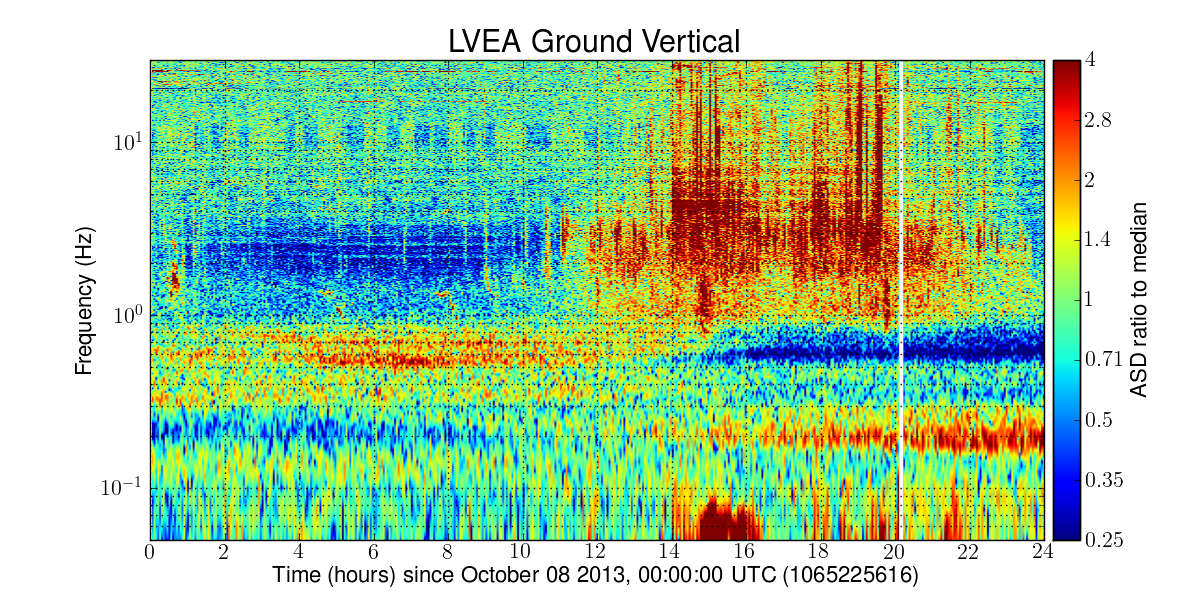
\includegraphics[width=\linewidth]{figures/Spectro_ground.png}
  \caption{Recent normalized spectrogram of Z-direction of ground motion sensors at Livingston}
  \label{fig:groundZspec}
\end{subfigure}%
\begin{subfigure}{.45\textwidth}
  \centering
  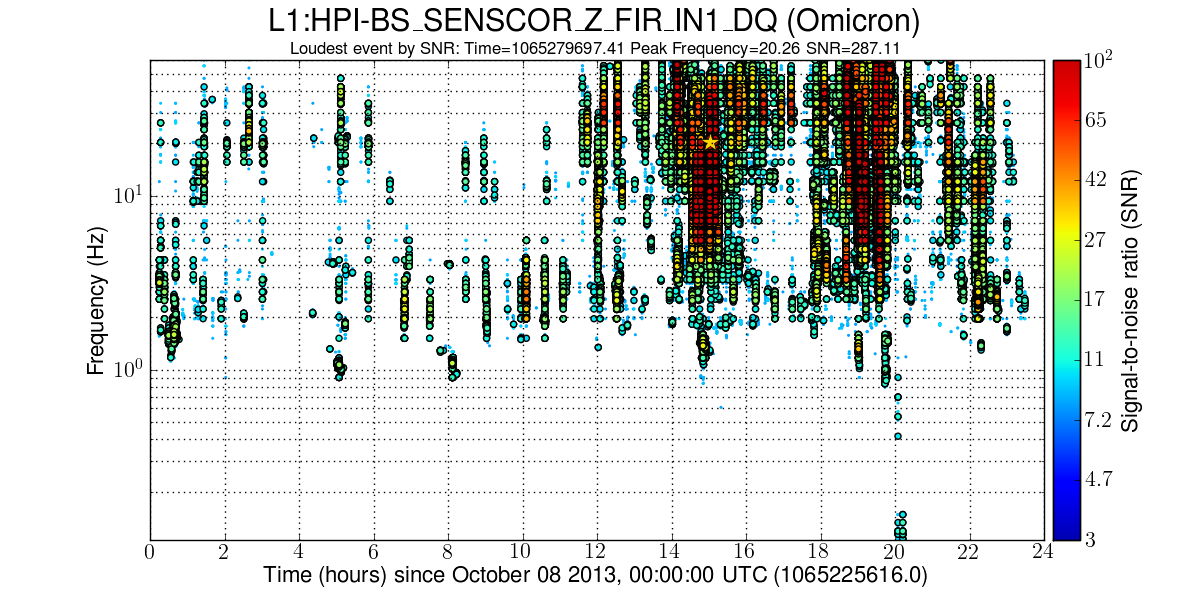
\includegraphics[width=\linewidth]{figures/Omicron_ground.png}
  \caption{Omicron triggers for the same channel during the same time period, before parameter tuning.}
  \label{fig:groundOmicron}
\end{subfigure}
\caption{A comparison of a recent normalized spectrogram of a Livingston ground motion sensor and Omicron triggers for the corresponding time - before parameter tuning. Note the low frequency structure seen below 1Hz in the normalized spectrogram is not seen by Omicron.}
\label{fig:OmicronTuning}
\end{figure}

Once Omicron is fully configured to resolve seismic transients, resolving transient noise in seismic sensor channels with good accuracy will be possible. I intend to use this tool in critical seismic transient studies (see~\S\ref{s:proposed}). 

All of these sensors have different units and ranges of validity. Tools used to analyze these channels for transient noise, or Event Trigger Generators, need to be tuned for each set of sensors in order to produce accurate trigger parameters like central time, frequency, and amplitude for transient events in these channels. 

\section{Techniques for transient noise mitigation}

%
%%
\subsection{Data quality vetoes}

\begin{figure}[htb]
	\center{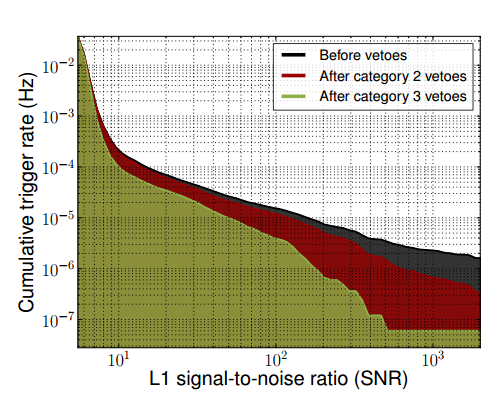
\includegraphics[scale=0.4]
	{figures/S6DQVetos.png}}
	\caption{\label{fig:S6DQ} An excerpt figure from the upcoming S6 detector characterization paper that draws heavily on the work I performed evaluating the performance of data quality flags, which are lists of time segments corresponding to pre-defined states of the detector. Data quality flags that indicate states where detection isn't possible are grouped together into 'categories' where lower category numbers indicate a more severe known problem. Categories 1 and 2 were removed from all transient \gw{} searches. Note the non-Gaussanity of this S6 Livingston distribution of single-detector burst search triggers after the removal of categories 1, 2 and 3.\todo{Check this is still current version of this figure with new detchar paper.}}
\end{figure}

%
%%
\subsection{Event-based veto generation}  

hveto, 




%%%%%%
%\subsection{Coherence studies} 
%
%A common follow-up to investigate potential couplings when the source of the noise is unknown is a coherence matrix, as shown in Figure \ref{fig:coherence}. For each matrix, the coherence between a list of interesting auxiliary channels indicative of potential noise couplings and the control signal (or channel of interest) is calculated for each 0.1 Hz frequency bin and plotted in a matrix form to easily spot potential correlations. Many configurations of this coherence matrix exist to target different subsystems, and I have developed those for the seismic isolation and suspensions systems. 
%
%As an example, the detector characterization group was recently requested by the Livingston site commissioners to investigate the source of unexpected excess noise below 1Hz in the PRMI signal.
%Our results (in Figure \ref{fig:coherence}) showed coherence of the ISI (Internal Seismic Isolation platforms) motion in HAM (auxiliary optics) chambers 2 and 3 and the suspension motion of optics in the same chamber with the PRMI control signal. The commissioners were able to use these results to isolate the problem and tune the ISI active seismic isolation loops to remove the excess noise. 
%
%\begin{figure}[htb]
%	\center{\includegraphics[scale=0.45]
%	{figures/CoherenceMatrix.png}}
%	\caption{\label{fig:coherence} Coherence of selected active seismic isolation platform motion sensors and suspension motion sensors with the PRMI control signal (PRCL) calculated for each 0.1 Hz wide frequency bin. Coherence with the PRMI signal was found for ISI (Internal Seismic Isolation platforms) motion and suspension motion in HAM (auxiliary optics) chambers 2 and 3 in the frequency range of the unknown noise source. } 
%\end{figure}

% --------------------------------------------------------------------------------------

%% -----------------------------------------------------------------------------------------
%% -----------------------------------------------------------------------------------------
%% -----------------------------------------------------------------------------------------
%% -----------------------------------------------------------------------------------------


